\documentclass[krantz2,ChapterTOCs]{krantz}
\usepackage{amssymb}
\usepackage{amsmath}
\usepackage{graphicx}
\usepackage{subfigure}
\usepackage{makeidx}
\usepackage{multicol}
\usepackage{listings}
\usepackage{xcolor}
\usepackage{hyperref}
\usepackage{url}
\usepackage{natbib}  % For APA-style citations
\usepackage{booktabs}
\usepackage{array}
\usepackage{enumitem}
\usepackage{comment}
\usepackage{float}
\usepackage[font=footnotesize,labelfont=bf]{caption}

% Tighten paragraph and section spacing
\setlength{\parskip}{0pt plus 1pt}
\setlength{\abovedisplayskip}{8pt plus 2pt minus 2pt}
\setlength{\belowdisplayskip}{8pt plus 2pt minus 2pt}

\makeindex

% preamble:
% Custom commands and macros for the chapter

% Change Bibliography to References
\renewcommand{\bibname}{References}

% Chapter abstract environment (krantz.cls provides none)
\newenvironment{abstract}%
  {\par\addvspace{6pt}\noindent\begingroup\small
   \textbf{Abstract:}\ \ignorespaces}%
  {\par\endgroup\addvspace{10pt}}

% Theorem-like environments
\newtheorem{theorem}{Theorem}[chapter]
\newtheorem{definition}{Definition}[chapter]
\newtheorem{example}{Example}[chapter]

% Code listing settings
\lstset{
    basicstyle=\ttfamily\footnotesize,
    breaklines=true,
    frame=single,
    backgroundcolor=\color{gray!10},
    keywordstyle=\color{blue},
    commentstyle=\color{green!50!black},
    stringstyle=\color{red!50!black},
    numbers=left,
    numberstyle=\tiny\color{gray},
    numbersep=5pt,
    tabsize=2,
    showstringspaces=false
}

% Python code environment
\lstnewenvironment{pythoncode}{
    \lstset{language=Python}
}{}

% Custom commands
\newcommand{\github}{\texttt{GitHub}}
\newcommand{\colab}{\texttt{Google Colab}}
\newcommand{\notebook}[1]{\texttt{\def\_{\textunderscore\allowbreak}#1}}
\newcommand{\package}[1]{\texttt{#1}}
\newcommand{\code}[1]{\texttt{#1}}

% Math operators
\DeclareMathOperator{\sigmoid}{sigmoid}
\DeclareMathOperator{\softmax}{softmax}
\DeclareMathOperator{\ReLU}{ReLU}

% Abbreviations
\newcommand{\ie}{i.e.,\ }
\newcommand{\eg}{e.g.,\ }
\newcommand{\cf}{cf.\ }
\newcommand{\etal}{et al.\ }

% =======================================

\begin{document}
\raggedbottom

\mainmatter

% Omit the front-matter table of contents (pages i--ii) but retain the
% \chapterauthor definition that krantz.cls normally installs via
% \tableofcontents.
\makeatletter
\gdef\chapterauthor{\@caplusone}
\makeatother

% For standalone chapter compilation
\setcounter{chapter}{21}



\chapterauthor{Arvid Lundervold}{Department of Biomedicine, University of Bergen, Bergen, Norway}

\chapter{Artificial Intelligence and Computational Medicine: A Hands-on Approach}
\label{ch:ai-compmed}

%% ============================================================================
\begin{abstract}
This chapter provides a hands-on, code-driven introduction to artificial intelligence in computational medicine, bridging the gap between theoretical understanding and practical implementation.
Covering three interconnected domains (medical imaging, multimodal data integration, and AI-assisted computing), we demonstrate current best practices using reproducible Jupyter notebooks with publicly available and synthetic datasets.
First, we address brain tumor segmentation from multiparametric MRI using a 3D U-Net trained with Dice loss, alongside promptable segmentation with the MedSAM2 foundation model.
Second, we present multimodal data integration through adaptive fusion networks that learn modality-specific importance weights, combined with graph neural networks operating on patient similarity networks for semi-supervised learning.
Third, we explore the role of large language models in medical research workflows, including text summarization, zero-shot classification, named entity recognition, and retrieval-augmented generation for grounding responses in verified evidence.
Throughout, we discuss key challenges: class imbalance, clinical interpretability, hallucination mitigation, missing modalities, privacy-preserving deployment, algorithmic fairness, and regulatory considerations.
All code, pretrained model weights, and materials are openly available, designed to run locally or on Google Colab, enabling researchers and clinicians to engage directly with working implementations.
\end{abstract}

%% ============================================================================
\section{INTRODUCTION}
\label{sec:introduction}

Artificial intelligence (AI) is transforming computational medicine, yet the gap between theoretical understanding and practical implementation remains a significant barrier for medical researchers and clinicians. 
This chapter provides a hands-on introduction through three interconnected domains (Figure~\ref{fig:workflow}): medical imaging analysis, multimodal data integration, and AI-assisted computing. 
Using reproducible Jupyter notebooks with publicly available and synthetic datasets, we demonstrate brain tumor segmentation with deep learning, patient similarity network (PSN) construction, and medical text analysis with large language models (LLMs). 
All code and materials are openly available at \url{https://github.com/arvidl/medAI-hands-on}, designed to run locally or on Google Colab.

The integration of AI into medicine represents one of the most significant technological shifts in healthcare~\citep{topol2019high, rajpurkar2022ai}. 
Deep learning has achieved remarkable performance in medical image analysis~\citep{esteva2019guide,lundervold2019overview}, with over 1,000 AI-based imaging tools now receiving FDA authorization~\citep{singh2025fda}. 
LLMs are transforming how we interact with medical knowledge~\citep{singhal2023large}, while multimodal approaches combining imaging, genomics, and clinical data promise more comprehensive patient characterization~\citep{acosta2022multimodal}.

\subsection{THE CURRENT LANDSCAPE}

Medical AI in 2026 occupies a distinctive position: mature enough for clinical deployment in specific domains, yet still evolving rapidly.
Three paradigm shifts characterize the current era:

\begin{description}[style=nextline, leftmargin=1em, labelindent=0pt, itemsep=0.2ex]
\item[From task-specific to foundation models]
Traditional deep learning required training separate models for each task (segmentation, classification, detection).
Foundation models like MedSAM~\citep{ma2025medsam2}, trained on millions of diverse medical images, can segment new anatomies with minimal prompting: a clinician draws a bounding box, and the model delineates the region of interest.
This shift dramatically reduces the annotation burden that has historically bottlenecked medical AI development.

\item[From siloed to multimodal integration]
Early clinical AI treated each data source independently: one model for chest X-rays, another for lab values, and a third for clinical notes.
Contemporary approaches integrate across modalities, using attention mechanisms and graph neural networks (GNNs) to capture complementary information.
Patient similarity networks (PSNs) represent patients as nodes in a graph, enabling community detection and semi-supervised learning that leverages relationships between patients.

\item[From static to agentic AI]
Initial LLM applications focused on single-turn interactions (summarization, classification).
Emerging agentic workflows chain multiple LLM calls with tool use, retrieval-augmented generation (RAG), and human-in-the-loop validation, moving toward AI systems that can reason through complex clinical scenarios while remaining grounded in verified evidence.
\end{description}

Despite these advances, a substantial gap persists between research and implementation. 
This chapter addresses these barriers through working code examples that readers can execute, modify, and extend.
All implementations are available as Jupyter notebooks in the accompanying GitHub repository; we reference specific notebooks using the format \notebook{notebook\_name.ipynb}.

This chapter presents three computational workflows. 
The first addresses brain tumor segmentation from multimodal magnetic resonance imaging (MRI) data~\citep{dorfner2025brain}. 
The second explores multimodal data integration through PSNs, enabling disease subtyping and personalized treatment recommendations~\citep{valous2024graph,lundervold2026psn} ({\small \url{https://github.com/arvidl/psn-ibs}}). 
The third examines the emerging role of LLMs in medicine, both for clinical text analysis and research workflows~\citep{raza2024generative}. Beyond research, LLMs show promise for patient-specific education, as demonstrated in diabetes care~\citep{skjervold2025diaguide}. 

Significant challenges remain, including model generalization across populations and clinical settings, evolving regulatory frameworks, and integration into clinical workflows requiring appropriate user interfaces and clear allocation of responsibility between clinicians and AI systems.

\begin{figure}[H]
\centering
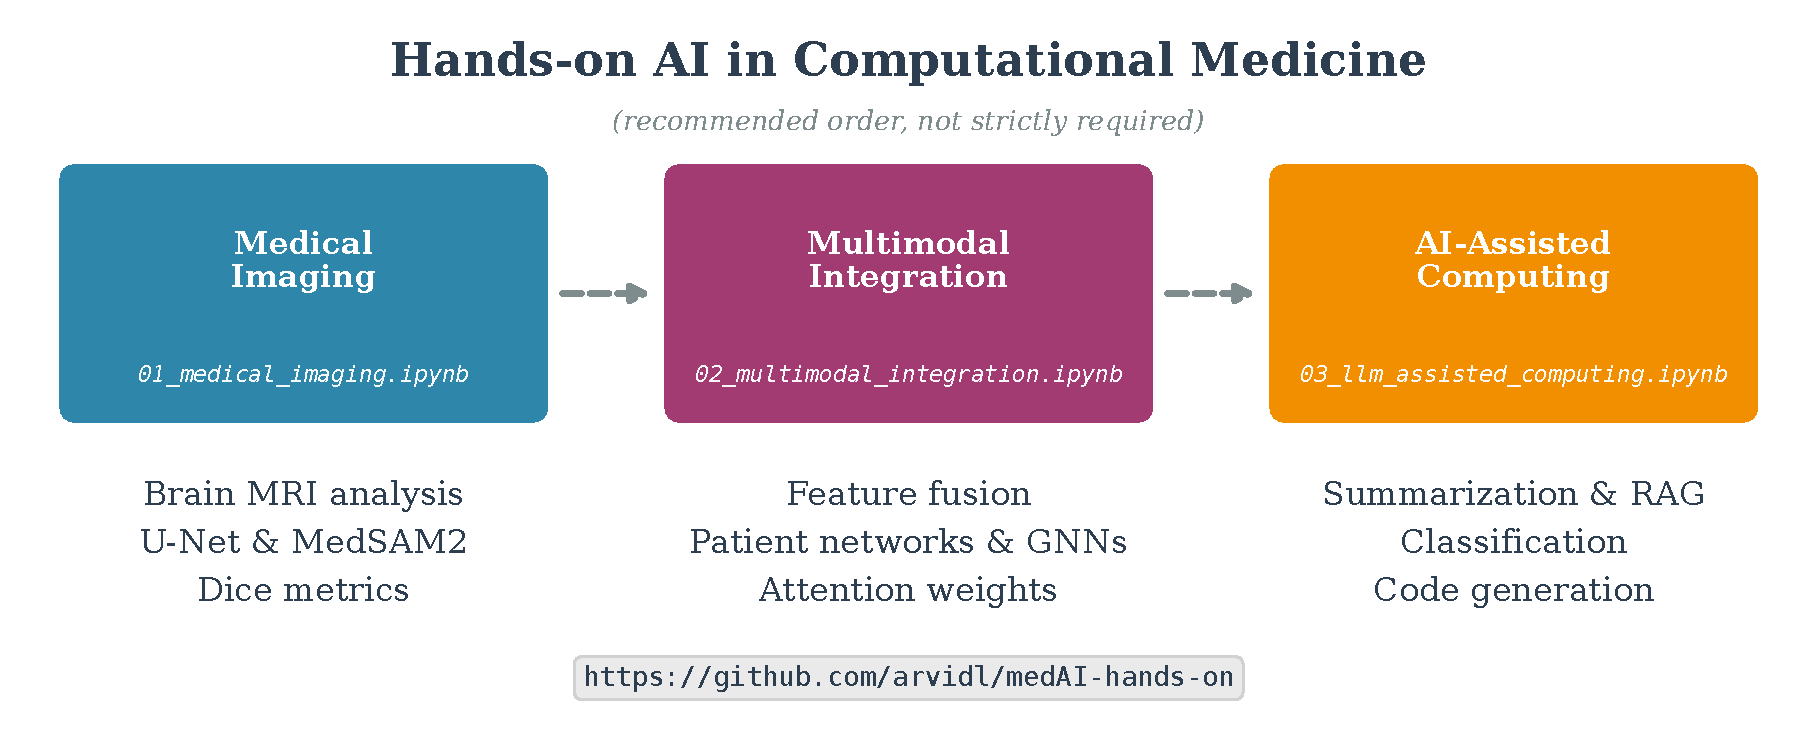
\includegraphics[width=0.95\textwidth]{figures/fig1_workflow.pdf}
\caption{Overview of the hands-on approach presented in this chapter. We cover three interconnected domains: (1)~medical imaging analysis with U-Net and MedSAM2 foundation models for brain tumor segmentation; (2)~multimodal data integration combining imaging and clinical features through adaptive fusion and graph neural networks on patient similarity networks; and (3)~AI-assisted computing using large language models with retrieval-augmented generation (RAG) for grounded responses. Each domain is accompanied by a Jupyter notebook that can be executed locally or on Google Colab.}
\label{fig:workflow}
\end{figure}

%% ============================================================================
\section{PREREQUISITES AND ENVIRONMENT SETUP}
\label{sec:setup}

We provide all materials through a public GitHub repository with setup instructions for local and cloud execution.

\subsection{COMPUTATIONAL REQUIREMENTS}

The examples are accessible across different computational resources:
\textbf{minimum}: CPU-only (slower but functional);
\textbf{recommended}: NVIDIA GPU with 8+ GB VRAM or Apple Silicon with MPS support;
\textbf{cloud}: Google Colab free tier with GPU access.
All notebooks include automatic device detection without user intervention.

\subsection{ENVIRONMENT SETUP}

For local execution, we provide a conda environment specification:

\begin{lstlisting}[language=bash,caption={Creating the conda environment}]
git clone https://github.com/arvidl/medAI-hands-on.git
cd medAI-hands-on
conda env create -f environment.yml
conda activate medai-handson
jupyter notebook
\end{lstlisting}

The environment includes PyTorch, MONAI for medical imaging~\citep{cardoso2022monai}, Hugging Face Transformers~\citep{wolf2020transformers}, PyTorch Geometric for GNNs~\citep{fey2019pyg}, and standard scientific Python libraries.
For Google Colab, notebooks include automatic dependency installation; users can open them directly via ``Open in Colab'' badges in the repository.

\subsection{DATA AND REPRODUCIBILITY}

The BraTS dataset ($\approx$900\,MB for 100 cases) is hosted on GitHub Releases and automatically downloaded at runtime.
All notebooks implement comprehensive seed-setting for reproducibility, with version-pinned dependencies and publicly available trained model weights.
Figures can be reproduced using \texttt{chapter/figures/generate\_figures.py}.

%% ============================================================================
\section{MEDICAL IMAGING: BRAIN TUMOR SEGMENTATION}
\label{sec:imaging}

Medical image segmentation, the task of delineating anatomical structures or pathological regions at the voxel level, is fundamental to computational medicine~\citep{lundervold2019overview}. 
We demonstrate brain tumor segmentation using the U-Net architecture~\citep{ronneberger2015unet}, a foundational model that has inspired variants, including nnU-Net~\citep{isensee2021nnu}.
We use data from the BraTS Challenge~\citep{menze2015brats}, specifically 100 cases from the Medical Segmentation Decathlon (70 train / 15 validation / 15 test), resized to $128^3$ voxels.

\subsection{THE BRAIN TUMOR SEGMENTATION TASK}

Gliomas present significant segmentation challenges due to heterogeneous appearance and infiltrative growth patterns. 
Multiparametric MRI provides complementary information~\citep{menze2015brats, bakas2017advancing}: T1-weighted images show anatomical detail; T1 with gadolinium contrast (T1-Gd) highlights active tumor regions; T2-weighted imaging reveals edema; and FLAIR suppresses cerebrospinal fluid (CSF) while preserving lesion contrast.
The segmentation task classifies each voxel into background, necrotic core, enhancing tumor, or peritumoral edema. 
Figure~\ref{fig:brain_seg} illustrates these modalities and segmentation results from our U-Net model.

\begin{figure}[H]
\centering
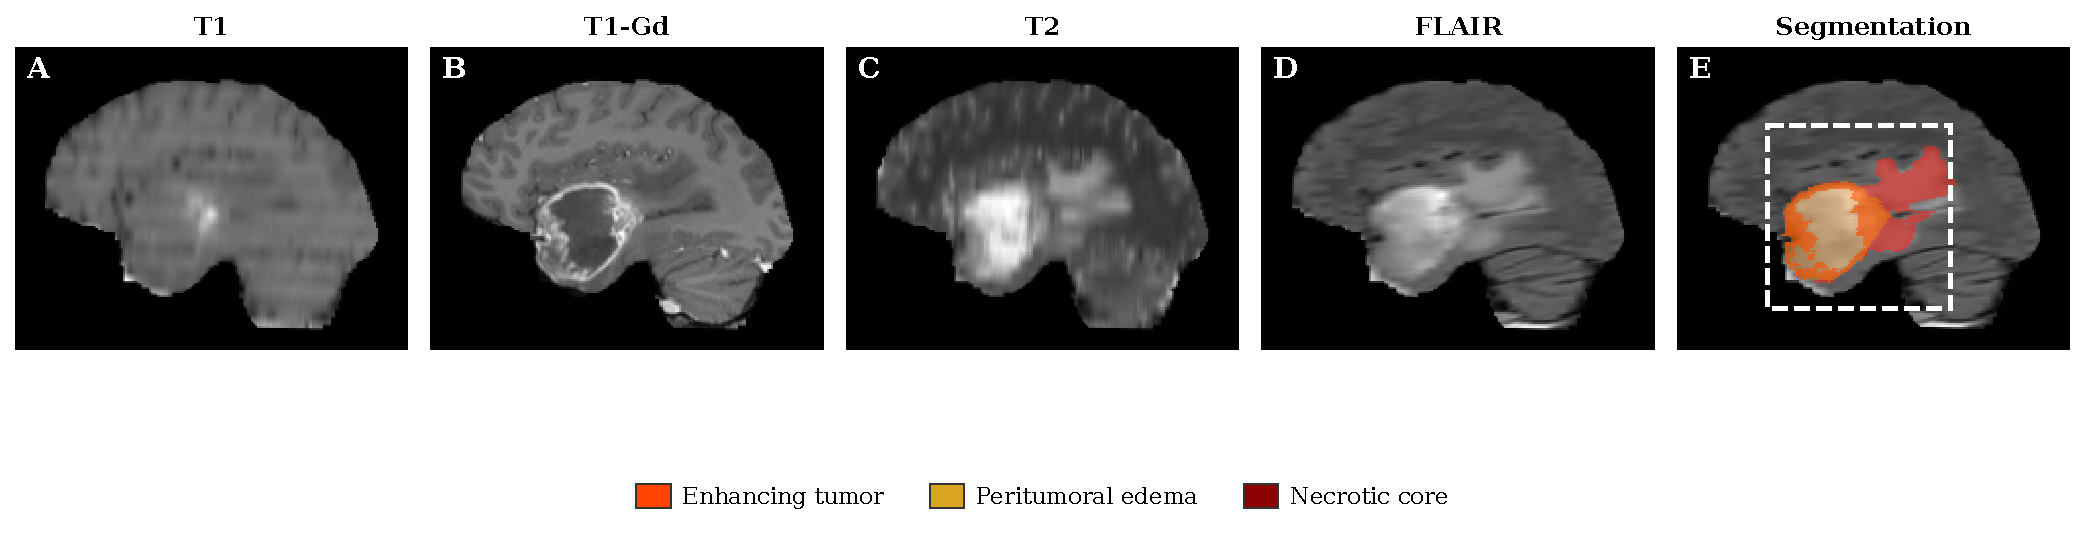
\includegraphics[width=0.95\textwidth]{figures/fig2_brain_mri.pdf}
\vspace{0.1cm}
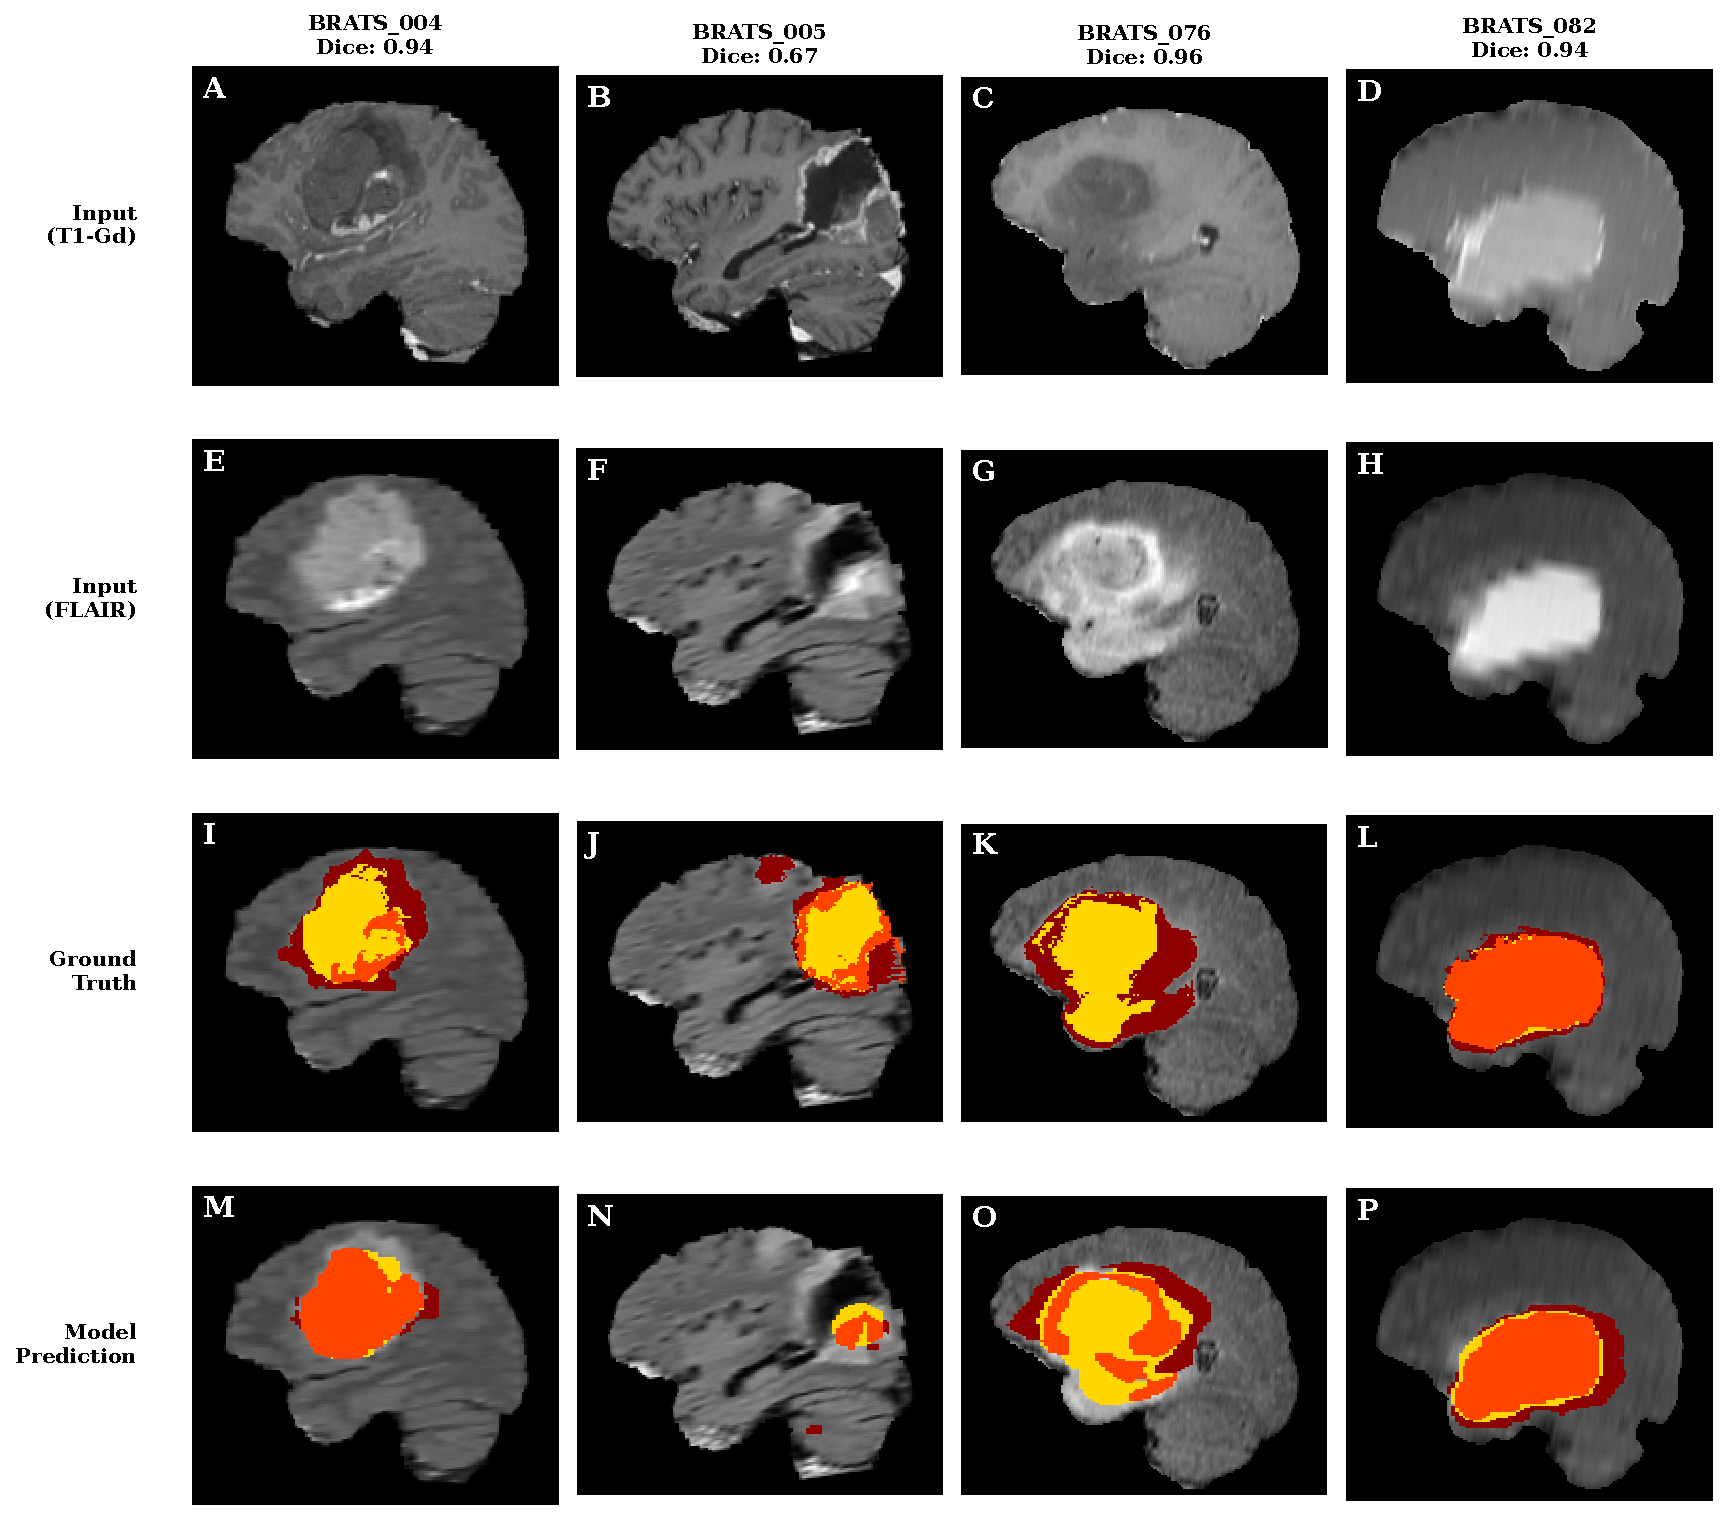
\includegraphics[width=0.95\textwidth]{figures/fig3_segmentation.pdf}
\caption{Brain tumor segmentation with multiparametric MRI. \textbf{Top panel (A--E)} depicts the four MRI sequences:
 T1 (A), T1-Gd (B), T2 (C), FLAIR (D) from case BRATS\_001 and expert segmentation overlay (E) showing tumor subregions: 
 enhancing tumor (orange), peritumoral edema (yellow), and necrotic core (red); dashed box indicates the tumor region of interest. 
\textbf{Bottom panel (A--P)} depticts segmentation results across four held-out test cases (columns). 
The four rows show T1-Gd input, FLAIR input, ground truth, and U-Net predictions, respectively. 
The model achieves Dice scores of 0.67--0.96, with performance varying by tumor characteristics: 
diffuse tumors (BRATS\_005, Dice: 0.67) are more challenging than well-defined cases (BRATS\_076, Dice: 0.96). 
The 3D U-Net (depth=4, 32 base features) was trained with early stopping on $128^3$ volumes.}
\label{fig:brain_seg}
\end{figure}

\subsection{THE U-NET ARCHITECTURE}

U-Net employs an encoder-decoder structure with skip connections~\citep{ronneberger2015unet}. 
The encoder downsamples through convolutions and pooling, capturing context at multiple scales; the decoder upsamples via transposed convolutions. 
Skip connections concatenate encoder and decoder features, combining semantic ``what'' information with spatial ``where'' information for accurate boundary delineation.
For 3D medical images, we use 3D convolutions to process full volumes.
The implementation is available in \texttt{src/models.py} and \notebook{01\_medical\_imaging.ipynb}.

\subsection{LOSS FUNCTIONS AND TRAINING}

Brain tumor segmentation exhibits severe class imbalance (tumors occupy 1--5\% of volume). 
The Dice loss addresses this by directly optimizing overlap:
\begin{equation*}
\mathcal{L}_{\text{Dice}} = 1 - \frac{2 \sum_{i} p_i g_i + \epsilon}{\sum_{i} p_i + \sum_{i} g_i + \epsilon}
\label{eq:dice}
\end{equation*}
where $p_i$ and $g_i$ are predicted probability and ground truth for voxel $i$.
Dice loss directly optimizes the overlap metric we care about, making it well-suited for imbalanced segmentation where cross-entropy would be dominated by the majority background class.

The training pipeline includes z-score intensity normalization within the brain region and data augmentation via random flips; additional augmentations (rotations, intensity variations, elastic deformations) can be added for improved generalization.
The complete pipeline with logging and early stopping is in \notebook{01\_medical\_imaging.ipynb}.

\subsection{EVALUATION AND EXTENSIONS}

Beyond Dice score, we evaluate sensitivity (critical for not missing tumor) and specificity.
For production use, consider nnU-Net~\citep{isensee2021nnu}, which automates preprocessing and architecture decisions; additional metrics such as Hausdorff distance (worst-case boundary error) are commonly used in clinical evaluation.

Extensions include multi-class segmentation, uncertainty estimation via Monte Carlo dropout, test-time augmentation, and transfer learning from larger public datasets.
For simplified workflows, fastMONAI~\citep{kaliyugarasan2023fastmonai} provides a low-code interface built on fastai and MONAI that streamlines model development for classification, regression, and segmentation tasks.\footnote{\url{https://github.com/MMIV-ML/fastMONAI}}

\subsection{FOUNDATION MODELS: MEDSAM2}

While supervised approaches like U-Net require task-specific training, \textbf{foundation models} offer an alternative paradigm: pretrained on massive, diverse datasets, they can segment new anatomies with minimal or zero additional training.
\textbf{MedSAM2}~\citep{ma2025medsam2} adapts Meta's SAM2 architecture for medical imaging, trained on 455,000+ 3D image-mask pairs across computed tomography (CT), MRI, positron emission tomography (PET), ultrasound, and endoscopy.
Rather than requiring full annotations, MedSAM2 uses \emph{bounding box or point prompts}: a clinician draws a box around the region of interest, and the model segments it, propagating across slices via memory attention.

Foundation models complement supervised training: use MedSAM2 for rapid prototyping and rare pathologies, or to generate pseudo-labels for training task-specific models.
\textcolor{blue}{In \notebook{01\_medical\_imaging.ipynb}, we contrast the supervised U-Net with a promptable MedSAM2 workflow on BraTS slices (real model when installed; otherwise a clearly labeled simulation). Full 3D memory-attention volume propagation is left as an extension using MedSAM2's video predictor API.}

%% ============================================================================
\section{MULTIMODAL DATA INTEGRATION}
\label{sec:multimodal}

Precision medicine increasingly relies on integrating multiple data modalities to achieve comprehensive patient characterization~\citep{acosta2022multimodal, huang2020fusion}. 
No single modality captures the complete picture: imaging reveals tumor characteristics, clinical variables provide treatment history, and genomics indicates molecular drivers. 
This section demonstrates multimodal fusion using imaging-derived features combined with clinical data, building on the segmentation workflow from Section~\ref{sec:imaging}.

\subsection{FROM SEGMENTATION TO FEATURES: THE CLINICAL AI PIPELINE}

This section builds directly upon Section~\ref{sec:imaging}, following a natural clinical AI pipeline. Once tumors are segmented, \textbf{radiomics pipelines} extract quantitative imaging features~\citep{aerts2014decoding}: shape descriptors (volume, sphericity, elongation), intensity statistics (mean, variance, skewness), and texture features (GLCM = gray-level co-occurrence matrix, GLRLM = gray-level run-length matrix) that capture spatial heterogeneity. These handcrafted features can be complemented by \textbf{deep features}, which are neural network embeddings from pretrained models that capture learned hierarchical representations, often extracted from encoder bottlenecks or foundation models~\citep{moor2023foundation}.

These imaging-derived features are then combined with clinical data (age, performance status, molecular markers such as isocitrate dehydrogenase (IDH) mutation and O\textsuperscript{6}-methylguanine-DNA methyltransferase (MGMT) promoter methylation) for survival prediction, treatment response assessment, or patient stratification~\citep{truhn2024oncology}.

For the demonstration notebook, we use synthetic data simulating radiomics-style imaging features (50 dimensions) combined with clinical variables (10 dimensions). 
This allows focus on integration methodology without requiring access to protected health information (PHI), while maintaining realistic correlation structures within feature groups.

\subsection{THE INTEGRATION CHALLENGE}

Different modalities present distinct challenges: dimensionality mismatch (imaging features outnumber clinical variables by orders of magnitude), scale heterogeneity (age in years vs.\ tumor volume in mm$^3$), missing data (incomplete clinical records, variable imaging protocols), and temporal misalignment (modalities acquired at different time points). We address these through \emph{a neural network architecture that learns modality-specific representations before fusion}~\citep{xu2023multimodal}, allowing each modality to be processed appropriately for its characteristics.

\subsection{ADAPTIVE FUSION ARCHITECTURE}

Rather than assuming equal contribution from imaging and clinical data, we learn relative modality importance dynamically (Figure~\ref{fig:multimodal}).
Given imaging features $\mathbf{x}_{\text{img}}$ and clinical features $\mathbf{x}_{\text{clin}}$, modality-specific encoders first map each to a shared latent space:
\begin{equation*}
\mathbf{z}_{\text{img}} = f_{\text{img}}(\mathbf{x}_{\text{img}}), \quad \mathbf{z}_{\text{clin}} = f_{\text{clin}}(\mathbf{x}_{\text{clin}})
\end{equation*}
where $f_{\text{img}}$ and $f_{\text{clin}}$ are small multilayer perceptrons (MLPs) producing $d$-dimensional embeddings.
A weighting network $g$ (a two-layer MLP with tanh activation) computes the \emph{adaptive fusion weights} $\alpha$ (imaging importance) and $\beta$ (clinical importance) from the concatenated representations:
\begin{equation*}
[\alpha, \beta] = \mathrm{softmax}\bigl(g([\mathbf{z}_{\text{img}}; \mathbf{z}_{\text{clin}}])\bigr), \quad \alpha + \beta = 1
\end{equation*}
The fused representation combines modalities according to learned importance:
\begin{equation*}
\mathbf{z}_{\text{fused}} = \alpha \cdot \mathbf{z}_{\text{img}} + \beta \cdot \mathbf{z}_{\text{clin}}
\end{equation*}
Finally, a classification MLP produces the output $\hat{y} = \mathrm{softmax}(\mathrm{MLP}(\mathbf{z}_{\text{fused}}))$.

The weights $(\alpha, \beta)$ provide interpretability: for each patient, we can examine whether the model relied more heavily on imaging or clinical features.
This transparency is valuable for clinical applications where understanding \emph{why} a prediction was made is as important as the prediction itself.
The implementation is in \notebook{02\_multimodal\_integration.ipynb}.

\subsection{PATIENT SIMILARITY NETWORKS}

An alternative approach to prediction-oriented fusion constructs PSNs~\citep{pai2018patient}.
Formally, a PSN is a graph $G = (V, E)$ where the node set $V = \{v_1, \ldots, v_n\}$ represents patients and edges $E$ encode pairwise similarity.
In a \emph{weighted graph}, each edge $(v_i, v_j)$ carries a weight $w_{ij} \in [0,1]$ reflecting similarity strength (e.g., cosine similarity of feature vectors).
In practice, we often threshold to obtain an \emph{unweighted graph}: $e_{ij} = 1$ if $w_{ij} > \tau$, else $0$, retaining only the most similar patient pairs.
This graph-based representation enables several clinical applications:

Applications include \emph{patient stratification} (community detection identifies subgroups with distinct prognoses), \emph{case-based reasoning} (retrieving similar historical cases to inform treatment decisions), and \emph{cohort visualization} (network layouts reveal population structure, outliers, and gradients not apparent from tabular data).

Figure~\ref{fig:multimodal} shows both the fusion architecture and a patient similarity network where patients cluster by outcome, demonstrating how multimodal integration captures clinically meaningful patient subgroups.

\subsection{GRAPH NEURAL NETWORKS FOR PATIENT SIMILARITY}

Beyond static similarity graphs, \textbf{GNNs} can learn directly on PSN structure~\citep{valous2024graph}.
GNNs encompass a family of architectures; we use \textbf{graph convolutional networks (GCNs)}, a widely adopted variant~\citep{kipf2017semi}.
Standard neural networks process each patient independently, ignoring relationships between cases.
GCNs instead leverage the graph structure: each patient's representation is iteratively refined by aggregating information from similar patients (its neighbors in the PSN).

GCNs formalize this as neighborhood aggregation.
At each layer $l$, patient $i$'s representation $\mathbf{h}_i \in \mathbb{R}^d$ (a $d$-dimensional vector) is updated by collecting and transforming neighbor representations:
\begin{equation*}
\mathbf{h}_i^{(l+1)} = \sigma\left(\sum_{j \in \mathcal{N}(i)} \frac{1}{\sqrt{d_i d_j}} \mathbf{W}^{(l)} \mathbf{h}_j^{(l)}\right)
\end{equation*}
where $\mathcal{N}(i)$ is the set of patients connected to $i$ in the PSN (i.e., those with similarity $w_{ij} > \tau$), $\mathbf{W}^{(l)} \in \mathbb{R}^{d \times d}$ is a learnable weight matrix that transforms features, $\sigma$ is a nonlinear activation (e.g., ReLU), and $d_i$ and $d_j$ are the node degrees, used to normalize messages so that highly connected nodes do not dominate.
Through stacked layers (each aggregating from immediate neighbors), information propagates multiple hops across the network: with $L$ layers, each patient's representation incorporates information from patients up to $L$ edges away.
A patient with unknown outcome can thus ``borrow'' information from similar patients with known outcomes, enabling \emph{semi-supervised learning}~\citep{kipf2017semi} where labeled and unlabeled patients jointly inform the model.

This is particularly valuable in medical settings where labeled outcomes are scarce, but unlabeled patient data is abundant.
\textcolor{blue}{In \notebook{02\_multimodal\_integration.ipynb}, we build a PSN on the same train/test node set used by the GCN and show that reasonable accuracy can be maintained even when only 50\% of training patients have labeled outcomes, illustrating label sharing through the similarity structure.}
The approach extends naturally to heterogeneous graphs incorporating multiple relationship types (shared diagnoses, similar treatments, comparable biomarker profiles).

\begin{figure}[H]
\centering
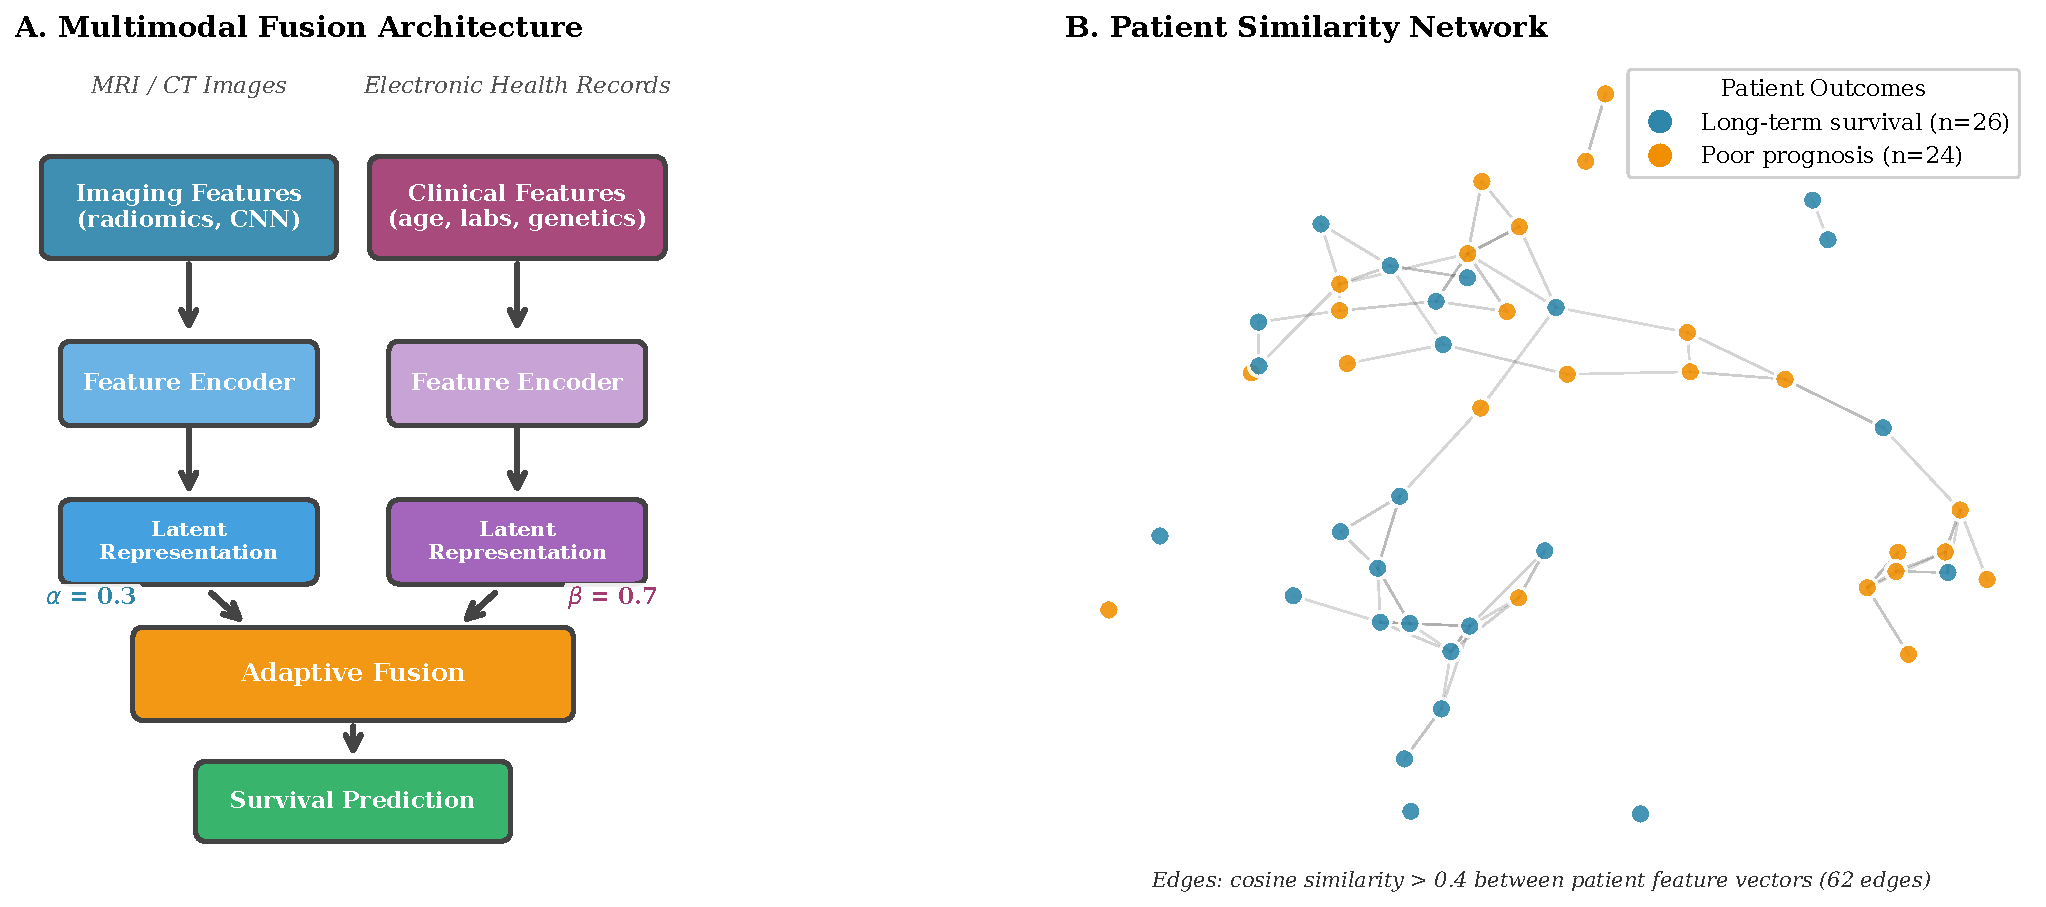
\includegraphics[width=0.95\textwidth]{figures/fig4_multimodal.pdf}
\caption{Multimodal data integration for brain tumor prognosis. \textbf{Panel~A:} Deep learning architecture with separate encoders for imaging features (radiomics) and clinical features (age, labs, genetics), transforming inputs into latent vectors. An adaptive fusion layer learns optimal weights ($\alpha$=0.3 imaging, $\beta$=0.7 clinical) for combining modalities. 
\textbf{Panel~B:} Patient similarity network (n=50 synthetic patients) constructed using the methodology from \texttt{02\_multimodal\_integration.ipynb}. Nodes colored by outcome (blue: long-term survival; orange: poor prognosis); edges connect patients with cosine similarity above 0.4. The network reveals two clusters corresponding to outcome groups.}
\label{fig:multimodal}
\end{figure}

\subsection{HANDLING MISSING MODALITIES}

A practical challenge in multimodal integration is missing data~\citep{wu2026missing}. Common strategies include: \emph{imputation} (replacing missing values with estimates such as mean, k-nearest neighbor, or learned networks), \emph{masking} (randomly dropping modalities during training so the model learns robustness), and \emph{late fusion} (computing modality-specific predictions independently, then combining only available modalities).

Our adaptive fusion architecture (Section~\ref{sec:multimodal}) supports masking during training and evaluation.
Consider a patient with imaging data but missing clinical records.
\textcolor{blue}{Zeroing $\mathbf{x}_{\text{clin}} = \mathbf{0}$ alone does not reliably drive the attention MLP to $\beta \approx 0$.
In \notebook{02\_multimodal\_integration.ipynb} we therefore combine modality dropout with \emph{presence masks}: a missing modality is zeroed and its fusion weight is forced to zero (renormalizing the remaining weight), so $\mathbf{z}_{\text{fused}} \approx \alpha \cdot \mathbf{z}_{\text{img}}$ with $\alpha = 1$ when clinical data are unavailable.}
For PSN construction, patients with missing modalities can still be included using available features, with similarity computed over the common feature space.

\subsection{EVALUATION AND CLINICAL UTILITY}

Multimodal models require evaluation beyond accuracy because they introduce complexity not present in single-modality approaches.
In brain tumor imaging, standard MRI sequences (T1, T1-Gd, T2, FLAIR) are acquired for all patients, but advanced sequences (perfusion MRI, MR spectroscopy) that improve differential diagnosis and treatment planning are not available at all centers or for all patients.
We must therefore answer: does the model degrade gracefully when advanced sequences are missing? Do standard sequences suffice for most patient subgroups?
Emerging \emph{radiogenomics} research suggests that mpMRI features may predict molecular markers (IDH mutation, MGMT methylation) when tissue is unavailable~\citep{sanchez2024radiogenomics, astaraki2026radiogenomics}, providing a potential fallback pathway for multimodal models.

Key evaluation dimensions include: \textbf{Calibration} (do predicted probabilities match empirical frequencies? A 70\% survival prediction should be correct $\sim$70\% of the time); \textbf{Decision curve analysis} (clinical utility across decision thresholds~\citep{vickers2006decision}); \textbf{Subgroup analysis} (does performance hold across demographics, disease stages, and modality availability?); and \textbf{Ablation studies} (systematically removing modalities to quantify each contribution; if performance is unchanged without a modality, that data source may be redundant).

%% ============================================================================
\section{AI-ASSISTED COMPUTING WITH LARGE LANGUAGE MODELS}
\label{sec:llm}

LLMs represent a paradigm shift in how we interact with medical knowledge~\citep{brown2020language, singhal2023large}. 
While direct clinical decision-making requires careful validation, LLMs offer immediate value for research workflows: literature summarization, information extraction, and code generation.
Recent systematic reviews provide evidence-based assessments of current maturity levels across application domains~\citep{artsi2025llmclinical}.

\subsection{APPLICATIONS AND MATURITY ASSESSMENT}

Current LLM applications in medicine vary substantially in maturity and readiness for clinical deployment. Table~\ref{tab:llm_maturity} summarizes evidence-based assessments across five key domains, reflecting the state of the field as of early 2026.

\begin{table}[t]
\centering
\caption{LLM Application Maturity in Medical Contexts (2026 Assessment). See text for supporting references.}
\label{tab:llm_maturity}
\small
\renewcommand{\arraystretch}{1.15}
\begin{tabular}{@{}>{\raggedright\arraybackslash}p{2.8cm}>{\raggedright\arraybackslash}p{3.2cm}>{\raggedright\arraybackslash}p{6.2cm}@{}}
\toprule
\textbf{Application} & \textbf{Status} & \textbf{Key Evidence} \\
\midrule
\textbf{Literature Review} & Operational Support & 85\% screening accuracy; 40\% time reduction in systematic reviews; emergence of PRISMA-trAIce reporting standards \\[1ex]
\textbf{Code Assistance} & Ubiquitous & 84\% developer adoption globally; 74\% autonomous fix rate on verified benchmarks; shift to agentic coding workflows \\[1ex]
\textbf{Report Drafting} & Regulated Production & $>$1,000 FDA authorizations in radiology; reinforcement learning (UniRG) effectively mitigates clinical hallucinations \\[1ex]
\textbf{Clinical Q\&A} & Deployed with Supervision & 75\% draft rate in major health systems; requires human-in-the-loop validation for patient-facing use \\[1ex]
\textbf{Diagnostic Support} & Advanced Decision Support & 94\% accuracy vs.\ 70.5\% human on image challenges; emergence of chain-of-thought reasoning agents \\
\bottomrule
\end{tabular}
\end{table}

\textbf{Code assistance} is most mature, with widespread developer adoption and strong performance on standard benchmarks. Agentic coding assistants (e.g., Cursor, GitHub Copilot, Google Antigravity, GPT-5 Codex, Lovable, Replit Agent) now autonomously implement multi-file changes, run tests, and iterate on feedback, or generate complete applications from prompts.
\textbf{Literature review} tools (e.g., Elicit, Consensus, Semantic Scholar, Rayyan, ASReview) achieve high screening accuracy with significant time reduction.
\textbf{Report drafting} is advancing rapidly, with ambient AI medical scribes (e.g., Nuance DAX, Abridge, DeepScribe, Noteless) automating clinical documentation.
\textbf{Clinical Q\&A} and \textbf{diagnostic support} show impressive capabilities but require human oversight for patient-facing use.

We demonstrate some of these capabilities in \notebook{03\_llm\_assisted\_computing.ipynb} using open-source models via Hugging Face Transformers~\citep{wolf2020transformers}, ensuring reproducibility without proprietary API access.

\subsection{DEMONSTRATED CAPABILITIES}

\begin{description}[style=nextline, leftmargin=1em, labelindent=0pt, itemsep=0.2ex]
\item[Summarization] Transformer models (BART, T5) condense lengthy medical documents, enabling rapid literature review. Given a multi-paragraph abstract, models produce concise summaries preserving key findings.

\item[Zero-shot classification] LLMs classify text into categories without task-specific training, leveraging semantic similarity between input text and category descriptions. This is valuable for literature categorization and clinical triage where labeled training data is scarce.

\item[Named entity recognition (NER)] Specialized models identify and extract medical concepts (symptoms, medications, diagnoses, procedures) from unstructured clinical text. This transforms free-text records into structured data suitable for downstream analysis, enabling applications such as automated coding, adverse event detection, and cohort identification from electronic health records.

\item[Question answering] Extractive QA identifies answer spans within documents, enabling intelligent literature search beyond keyword matching. Combined with retrieval systems, this accelerates evidence synthesis.

\item[Code generation] LLMs assist with analysis scripts, particularly valuable for researchers with domain expertise but limited programming experience. Generated code should always be reviewed before execution.
\end{description}

\noindent Complete examples are in \notebook{03\_llm\_assisted\_computing.ipynb}.

\subsection{HALLUCINATION MITIGATION STRATEGIES}

A critical barrier to clinical LLM deployment has been hallucination, the generation of plausible but factually incorrect statements. Several mitigation strategies have emerged:

\begin{description}[style=nextline, leftmargin=1em, labelindent=0pt, itemsep=0.2ex]
\item[Retrieval-Augmented Generation (RAG)] Ground LLM responses in retrieved documents from verified sources (clinical guidelines, peer-reviewed literature), reducing reliance on parametric memory that may contain errors. We demonstrate a complete RAG implementation in \notebook{03\_llm\_assisted\_computing.ipynb}, using ChromaDB for vector storage and sentence transformers for embeddings.

\item[Chain-of-Thought Reasoning] Prompting models to explicitly show reasoning steps enables verification of the logical path to conclusions and often improves accuracy on complex medical queries. Current frontier models incorporate this capability natively as ``extended thinking'' modes (e.g., GPT-5 with reasoning, Claude extended thinking, Gemini Deep Think), where the model performs deliberate multi-step reasoning before responding~\citep{wei2022chainofthought}. These reasoning models achieve substantially higher accuracy on complex analytical tasks by allocating additional inference-time computation.

\item[Reinforcement Learning from Clinical Feedback] The UniRG framework~\citep{liu2026unirg} demonstrates that training with clinical reward signals (explicitly penalizing hallucinations and rewarding accurate diagnostic findings) substantially reduces clinically significant errors compared to standard text-generation objectives optimized for linguistic fluency.

\item[Calibrated Confidence Scores] Training models to output well-calibrated uncertainty estimates enables flagging of low-confidence outputs for mandatory human review~\citep{savage2025llmuncertainty,liu2025uqsurvey}.

\item[Human-in-the-Loop Validation] For clinical applications, treating all LLM outputs as drafts requiring expert validation remains essential. This includes structured review workflows with audit trails documenting AI contributions~\citep{alu2026auditableai,kolbinger2025adaptivevalidation}.
\end{description}

\subsection{PRIVACY AND DEPLOYMENT CONSIDERATIONS}

\begin{description}[style=nextline, leftmargin=1em, labelindent=0pt, itemsep=0.2ex]
\item[Cloud models] (GPT-5, Claude, Gemini) offer state-of-the-art performance but raise privacy concerns for PHI. Cloud providers typically prohibit PHI in terms of service. In the US, HIPAA (Health Insurance Portability and Accountability Act) compliance requires careful consideration of business associate agreements; similar regulations apply in other jurisdictions (e.g., GDPR in Europe, PIPEDA in Canada).

\item[Local models] (Llama, Mistral, BioMistral) run entirely on institutional hardware, ensuring data never leaves the institution. Recent advances in quantization (8-bit, 4-bit weights) have made running capable 7B--70B parameter models on consumer GPUs feasible. For medical institutions, local deployment may be the only option compatible with data governance requirements.

\item[Hybrid approaches] process sensitive data locally while using cloud application programming interfaces (APIs) for non-sensitive tasks. De-identification pipelines can remove PHI before cloud processing, though residual re-identification risks remain.
\end{description}

Figure~\ref{fig:llm_pipeline} illustrates an LLM-assisted workflow incorporating human validation.

\begin{figure}[H]
\centering
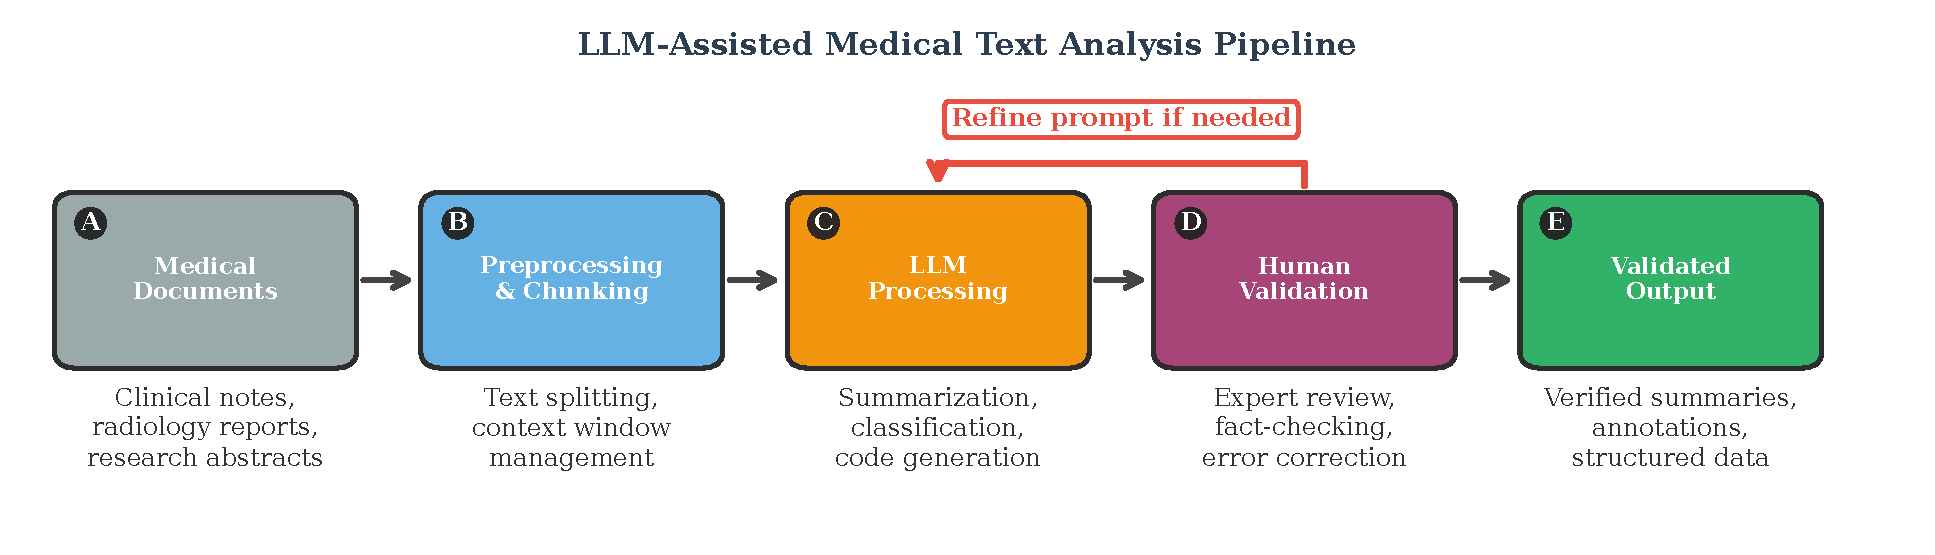
\includegraphics[width=0.95\textwidth]{figures/fig5_llm_pipeline.pdf}
\caption{Workflow for LLM-assisted medical text analysis. \textbf{(A)}~Medical documents including clinical notes and research abstracts. 
\textbf{(B)}~Preprocessing: text chunking for context windows. 
\textbf{(C)}~LLM processing: summarization, classification, or code generation. 
\textbf{(D)}~Human validation: expert review for accuracy and hallucinations. 
\textbf{(E)}~Validated output. 
The feedback loop indicates iterative prompt refinement (multi-turn interaction). Human oversight is essential; LLM outputs should never be used for patient care without verification.}
\label{fig:llm_pipeline}
\end{figure}

%% ============================================================================
\section{DISCUSSION AND BEST PRACTICES}
\label{sec:discussion}

Having demonstrated practical implementations across three domains, we synthesize lessons learned and best practices for medical AI development.

\subsection{COMPUTATIONAL OPTIMIZATION}

Efficient use of computational resources is crucial for accessibility.
Key techniques include \emph{mixed precision training} (reducing memory by up to 50\% with negligible quality impact), \emph{gradient checkpointing} (trading computation for memory to enable larger models), \emph{model quantization} (8-bit or 4-bit weights for efficient LLM deployment), and leveraging \emph{pretrained models} to reduce training time and data requirements.

\subsection{HANDLING CLASS IMBALANCE}

Medical datasets frequently exhibit severe class imbalance (rare diseases, small lesions, adverse events).
Strategies include \emph{loss function design} (Dice loss, focal loss~\citep{lin2017focal}, class-weighted cross-entropy), \emph{sampling strategies} (oversampling minority classes, balanced batches), and appropriate \emph{evaluation metrics} (sensitivity/specificity, AUROC = area under the receiver operating characteristic curve, AUPRC = area under the precision--recall curve rather than accuracy, which is misleading for imbalanced data).

\subsection{CLINICAL INTERPRETABILITY}

For clinical adoption, understanding model predictions is often as important as accuracy.
\emph{Attention visualization} (Grad-CAM = gradient-weighted class activation mapping~\citep{selvaraju2017grad} for imaging, modality weights for multimodal) highlights influential regions and data sources.
\emph{Feature importance} via SHapley Additive exPlanations (SHAP) values~\citep{lundberg2017shap} quantifies each variable's contribution to individual predictions.
\emph{Uncertainty quantification} (Monte Carlo dropout, ensembles) flags unreliable predictions requiring human oversight~\citep{huang2024uqreview,lopez2025uqsurvey}.
\emph{Concept-based explanations} express predictions in clinically meaningful terms (``high tumor heterogeneity'') rather than raw features.

\subsection{REPRODUCIBILITY CHECKLIST}

We recommend the following practices for reproducible medical AI research:
(1)~Version control all code using Git with tagged releases;
(2)~Specify exact package versions in environment files;
(3)~Set random seeds for all sources of randomness;
(4)~Document data preprocessing steps in detail;
(5)~Provide trained model weights and configuration files;
(6)~Use containerization (Docker) for complex environments;
(7)~Report metrics with confidence intervals across multiple runs;
(8)~Make code and data available through persistent repositories.

Several reporting standards promote transparency and trust in medical AI.
\emph{Model cards}~\citep{mitchell2019modelcards} provide standardized documentation of a model's purpose, performance across demographic groups, intended use cases, and limitations.
\emph{TRIPOD+AI}~\citep{collins2024tripodai} offers updated guidance for reporting clinical prediction models developed using machine learning, with a 27-item checklist covering data, methods, and evaluation.
\emph{SPIRIT-AI} and \emph{CONSORT-AI}~\citep{liu2020consortai} extend clinical trial reporting standards for AI interventions, ensuring transparent description of AI components, human-AI interaction, and failure case analyses.
Adopting these standards facilitates peer review, replication, and clinical translation.

\subsection{AI IN MEDICAL EDUCATION AND RESEARCH}

The integration of AI is transforming both medical education and research workflows, creating new opportunities and challenges for training the next generation of physician-scientists.

\begin{description}[style=nextline, leftmargin=1em, labelindent=0pt, itemsep=0.2ex]
\item[Transforming medical education]
AI is reshaping how medical students and residents learn.
Intelligent tutoring systems provide personalized learning paths based on individual performance patterns.
LLM-powered platforms can generate case studies, explain complex concepts in multiple ways, and engage in Socratic dialogue about diagnostic reasoning.
Virtual patients with AI-driven responses enable practice of clinical communication without risk.
Patient-specific education tools, such as those demonstrated for diabetes self-management~\citep{skjervold2025diaguide}, show how AI can tailor health information to individual contexts.

However, AI in education raises concerns about over-reliance on automated feedback, potential reinforcement of biases present in training data, and the importance of maintaining human mentorship and clinical intuition that cannot be reduced to pattern recognition.

\item[Accelerating research workflows]
For researchers, AI tools have become integral to daily practice.
Literature review is accelerated by summarization models; hypothesis generation is informed by knowledge graph analysis; code generation assists with analysis pipelines.
The RAG-based systems demonstrated in \notebook{03\_llm\_assisted\_computing.ipynb} exemplify how researchers can ground LLM interactions in verified literature, reducing hallucination risk while maintaining efficiency gains.

\item[Computational literacy as core competency]
As AI permeates medicine, computational literacy becomes essential for clinicians and researchers alike.
Understanding model limitations, recognizing when AI predictions should be questioned, and knowing how to validate outputs are skills as important as interpreting laboratory values or imaging studies.
The hands-on approach advocated in this chapter (working with code, examining model behavior, understanding failure modes) builds this literacy more effectively than passive learning.
\end{description}

\subsection{ETHICAL CONSIDERATIONS AND GOVERNANCE}

AI in medicine raises important ethical considerations that increasingly influence regulatory approval and institutional adoption:

\begin{description}[style=nextline, leftmargin=1em, labelindent=0pt, itemsep=0.2ex]
\item[Informed consent] Patients should understand when AI is involved in their care and have the opportunity to opt out where appropriate. Transparency about AI use builds trust and respects patient autonomy.

\item[Algorithmic fairness] Models may perform differently across demographic groups due to training data imbalances. Evaluation stratified by race, ethnicity, sex, age, and socioeconomic factors helps identify and mitigate disparities before deployment.

\item[Explainability requirements] High-stakes decisions (cancer diagnosis, treatment selection) demand explanations that clinicians and patients can understand. Black-box predictions may be unacceptable for consequential medical decisions, even if technically accurate.

\item[Human oversight] AI should augment rather than replace clinical judgment. Appropriate human-AI teaming preserves clinician accountability while leveraging AI's pattern recognition capabilities. The EU AI Act and FDA guidance increasingly require human-in-the-loop for high-risk applications.

\item[Continuous monitoring] Deployed models require ongoing surveillance for performance drift, particularly as patient populations, clinical practices, and data sources evolve. Establishing feedback loops for error reporting and model updating is essential for safe long-term deployment.
\end{description}

%% ============================================================================
\section{CONCLUSIONS}
\label{sec:conclusions}

This chapter presented a hands-on approach to AI in computational medicine across three domains: medical image segmentation, multimodal data integration, and AI-assisted computing with LLMs.
For \emph{deep learning segmentation}, U-Net with Dice loss achieves competitive performance even with modest resources, while foundation models like MedSAM2 enable promptable segmentation without task-specific training.
For \emph{multimodal fusion}, adaptive networks enable comprehensive patient characterization with interpretable modality weighting, and GNNs on patient similarity structures leverage unlabeled data through semi-supervised learning.
For \emph{large language models}, RAG grounds responses in verified evidence, mitigating hallucination in summarization, classification, and code generation tasks.
Throughout, executable notebooks and pretrained weights lower barriers to entry, while careful seed management ensures \emph{reproducible} results across platforms.

\subsection{FUTURE DIRECTIONS AND PERSPECTIVES}

The field of medical AI continues to evolve rapidly. Several trends will shape its trajectory over the coming years:

\begin{description}[style=nextline, leftmargin=1em, labelindent=0pt, itemsep=0.2ex]
\item[Foundation models for medical imaging]
Models like MedSAM2~\citep{ma2025medsam2}, trained on hundreds of thousands of 3D medical volumes, represent a paradigm shift from task-specific training.
\textcolor{blue}{We demonstrated promptable segmentation in \notebook{01\_medical\_imaging.ipynb} (bounding-box prompts on MRI slices); extending this to automatic propagation across entire volumes via memory attention is a natural next step with MedSAM2's 3D/video predictor.}
Future developments will extend this to multimodal foundation models integrating imaging, pathology, and clinical text, potentially enabling zero-shot diagnosis from minimal examples.

\item[Graph-based learning at scale]
The GNN approach demonstrated for PSNs extends naturally to larger knowledge graphs integrating disease ontologies, drug interactions, and molecular pathways~\citep{wang2024knowddi}.
Healthcare institutions are beginning to construct institutional patient graphs spanning millions of encounters, enabling discovery of treatment patterns and outcome predictors invisible to traditional analysis.

\item[Federated and privacy-preserving learning]
Multi-institutional collaboration remains essential for developing generalizable models, yet data sharing faces privacy barriers~\citep{teo2024federated}.
Federated learning trains models across institutions without centralizing data, while differential privacy provides formal guarantees against re-identification.
Synthetic data generation offers another pathway~\citep{giuffre2023synthetic}: generative models (GANs, VAEs = variational autoencoders, diffusion models) create realistic but artificial patient records that preserve statistical properties of the original data while eliminating re-identification risks, enabling models trained on synthetic data to be shared freely across institutions.

\item[Agentic AI workflows]
Moving beyond single-turn LLM interactions, agentic systems chain multiple reasoning steps with tool use (database queries, literature search, calculation).
The RAG implementation in \notebook{03\_llm\_assisted\_computing.ipynb} represents a building block; full agents might retrieve evidence, reason about applicability, request additional tests, and draft recommendations, all with human oversight at critical junctures.

\item[Regulatory evolution]
The EU AI Act classifies most diagnostic AI as high-risk, requiring conformity assessments, human oversight, and transparent documentation~\citep{aboy2024euaiact}.
FDA's evolving framework for AI/ML-based software as a medical device (SaMD) increasingly accommodates adaptive algorithms while maintaining safety standards.
Understanding these regulatory landscapes becomes essential for developers and deployers alike.

\item[The human-AI interface]
Perhaps the most critical challenge is designing effective human-AI collaboration~\citep{tun2025aitrust}.
Research on appropriate trust calibration, decision support interfaces, and workflow integration determines whether AI augments or disrupts clinical practice.
The goal is neither full automation nor trivial assistance, but genuine partnership where each party contributes complementary strengths.

\item[Data sharing and interoperability]
FAIR (Findable, Accessible, Interoperable, Reusable) data principles are increasingly central to medical AI development and validation.
The FUTURE-AI international consensus guideline~\citep{lekadir2025futureai} provides a framework for trustworthy and deployable healthcare AI, addressing clinical, technical, ethical, and legal considerations.
Standardization efforts around Fast Healthcare Interoperability Resources (FHIR) and Observational Medical Outcomes Partnership (OMOP) enable cross-institutional model development and validation, though interoperability remains the primary obstacle to full FAIR compliance.

\item[Sustainable and local AI]
The environmental footprint of large AI models raises ethical questions about balancing medical benefits against energy consumption and carbon emissions~\citep{schmitz2026sustainableai}.
Local deployment of quantized models (Llama, Mistral) addresses both privacy requirements and sustainability concerns, reducing dependence on energy-intensive cloud infrastructure.
Efficient architectures and training strategies become increasingly important as medical AI scales.

\item[Emerging computational paradigms]
Neuro-symbolic AI combines neural pattern recognition with symbolic reasoning, enabling more auditable and explainable healthcare applications~\citep{prenosil2025neurosymbolic,bhuyan2024neurosymbolic}.
Causal machine learning~\citep{feuerriegel2024causal} moves beyond correlation to predict treatment outcomes under different interventions, addressing a fundamental limitation of traditional predictive models.
Neuromorphic computing, inspired by biological neural architectures, promises energy-efficient inference for edge deployment in resource-constrained clinical settings.

\item[Global health equity]
AI risks widening health disparities if algorithms trained on data from high-income populations perform poorly in underrepresented groups~\citep{dychiao2024aihealthequity}.
Strategies for equitable AI include establishing Centres of Excellence in low- and middle-income countries~\citep{akbarialiabad2024lmicai}, developing locally relevant training datasets, and ensuring participatory design processes that center community needs.
Bridging the digital divide requires attention to infrastructure, connectivity, and contextually appropriate solutions.
\end{description}

\subsection{CLOSING REMARKS}

Medical AI occupies a unique position at the intersection of computer science, clinical medicine, and ethics, where stakes involve human health, regulatory requirements, and the clinician-patient relationship.
The techniques demonstrated here represent current best practices, yet the field advances rapidly; what endures is the approach of hands-on engagement with working code, critical evaluation of model outputs, and awareness of both capabilities and limitations.

Materials at \url{https://github.com/arvidl/medAI-hands-on} provide a foundation for further exploration.
By understanding these fundamentals through working implementations, readers are prepared to engage with medical AI as developers, researchers, educators, or clinicians.
The path forward requires collaboration across disciplines, and this chapter offers one entry point into that endeavor.

%% ============================================================================
%% Acknowledgments (optional)
%\section*{Acknowledgments}
%The author thanks...


{\footnotesize
\bibliographystyle{apalike}
\bibliography{references}
}

\end{document}
